%
% 1_Idee.tex -- Abschnitt 1 Grundidee der Sylvester-Matrix
%
% (c) 2026 Jakob Gierer, OST Ostschweizer Fachhochschule
%
% !TEX root = ../../buch.tex
% !TEX encoding = UTF-8
%
\section{Grundlegende Idee
\label{resultante:section:Idee}}
\kopfrechts{Grundlegende Idee}
Haben die Polynome \(f(X)=f_mX^m+\dots+f_1X+f_0\) mit \(\deg(f)=m\)
und \(g(X)=g_nX^n+\dots+g_1X+g_0\) mit \(\deg(g)=n\) einen gemeinsamen
Teiler \(d(X)\), dessen Grad mindestens \(1\) ist?

\noindent
Falls ja, dann gibt es Polynome \(p(X)\) und \(q(X)\) mit
\begin{equation}
    f(X)=q(X)\cdot d(X)\quad \text{und} \quad
    g(X)=p(X)\cdot d(X)
    \label{resultante:equation:divisor}
\end{equation}
mit \(\deg (d) \geq 1\), \(\deg(q)<\deg(f)\) und \(\deg(p)<\deg(g)\).

Aus (\ref{resultante:equation:divisor}) folgt
\begin{equation}
    \deg (q) = \deg (f) - \deg (d) \leq m-1 \quad \text{und} \quad
    \deg (p) = \deg (g) - \deg (d) \leq n-1.
\end{equation}
Das Polynom (\ref{resultante:equation:divisor}) links wird mit \(p(X)\)
multipliziert und das Polynom (\ref{resultante:equation:divisor}) rechts
mit \(q(X)\).
Aus diesen erweiterten Polynomen wird die Differenz
\begin{equation}
    fp-gq=0
    \label{resultante:equation:lgs}
\end{equation}
gebildet.
Daraus lässt sich eine Gleichung für die Koeffizienten von \(p\)
und \(q\) gewinnen.
Da der Grad von \(d(X)\) vorher nicht bekannt ist, wird hier mit dem
kleinsten Grad von \(d(X)\) weiterverfahren.
Sollte \(\deg d(X)=2\) sein, so werden die höchsten Koeffizienten von
\(q(X)\) und \(p(X)\) einfach \(0\).
\begin{figure}
    \centering
    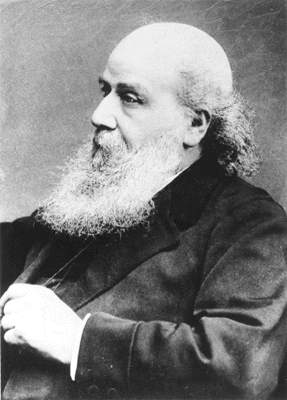
\includegraphics[width=0.4\textwidth]{papers/resultante/pictures/jjsylvester.png}
    \caption{Der britische Mathematiker James Joseph Sylvester \cite{resultante:jjsylvester}.}
\index{Sylvester, James Joseph}%
    \label{resultante:fig:jjsylvester}
\end{figure}
\begin{beispiel}
    Für die Polynome \(f(X)=2X^3+7X^2-5X-4\) und \(g(X)=2X^2+X-3\) werden
    die um Grad \(1\) kleineren Hilfspolynome \(q(X)=q_2X^2+q_1X+q_0\)
    und \(p(X)=p_1X+p_0\) bestimmt.
    Diese werden nun in (\ref{resultante:equation:lgs}) eingesetzt und
    nach den Koeffizienten absteigend sortiert, daraus resultiert die
    Polynomgleichung
    \begin{equation}
        \begin{aligned}
            (2p_1-2q_2)& X^4+\\
            (7p_1+2p_0-q_2-2q_1)& X^3+\\
            (-5p_1+7p_0+3q_2-q_1-2q_0)& X^2+\\
            (-4p_1-5p_0+3q_1-q_0)& X^{\phantom{0}}+\\
            (-4p_0+3q_0)& \phantom{X^0}=0.
        \end{aligned}
        \label{resultante:equation:gs}
    \end{equation}
    Dass in (\ref{resultante:equation:gs}) alle Koeffizienten
    verschwinden, kann als Gleichungssystem in der Matrixform
    \begin{equation}
        \begin{pmatrix}
            p_1&p_0&-q_2&-q_1&-q_0
        \end{pmatrix}
        \,
        \begin{pmatrix*}[r]
            2 &\phantom{-}7 & -5 & -4 &  0 \\
            0 &           2 &  7 & -5 & -4 \\
            2 &           1 & -3 &  0 &  0 \\
            0 &           2 &  1 & -3 &  0 \\
            0 &           0 &  2 &  1 & -3
        \end{pmatrix*}=0
        \label{resultante:equation:Syl}
    \end{equation}
    für die Koeffizienten der Hilfspolynome \(q(X)\) und
    \(p(X)\) geschrieben werden. Die Systemmatrix der Gleichung
    (\ref{resultante:equation:Syl}) ist die Sylvester-Matrix,
    benannt nach dem britischen Mathematiker James Joseph Sylvester
    (Abb.~\ref{resultante:fig:jjsylvester}).
    \label{resultante:beispiel:lgs}
\end{beispiel}
Die Idee der Umformungsschritte bis hierher ist, eine Übersicht zu
bekommen, woher die Sylvester-Matrix kommt.

\subsection{Die Sylvester-Matrix
\label{resultante:subsection:Sylvester-Matrix}}
Für zwei Polynome kann die in (\ref{resultante:equation:Syl}) gefundene
Matrix wie folgt allgemein definiert werden.

\begin{definition}[Sylvester-Matrix]
\index{Sylvester-Matrix}%
    Seien \(a(X)=a_nX^n+a_{n-1}X^{n-1}+\dots+a_1X+a_0\) und
    \(b(X)=b_mX^m+b_{m-1}X^{m-1}+\dots+b_1X+b_0\) Polynome vom Grad
    \(\deg a=n\) beziehungsweise \(\deg b=m\).
    Die \emph{Sylvester-Matrix} von a und b ist die \((n + m) \times
    (n + m)\)-Matrix:
    % \begin{equation}
        
    %     \begin{pmatrix}
    %         a_n&a_{n-1}&a_{n-2}&\dots&&&&&\\
    %         &a_n&a_{n-1}&a_{n-2}&\dots&&&&\\ 
    %         &&a_n&a_{n-1}&a_{n-2}&\dots&&&\\
    %         &&&\ddots&\ddots&\ddots&\ddots&&\\
    %         &&&&&\dots&a_1&a_0&\\
    %         &&&&&&\dots&a_1&a_0\\ \hdashline
    %         b_m&b_{m-1}&b_{m-2}&\dots&&&&&\\
    %         &b_m&b_{m-1}&b_{m-2}&\dots&&&&\\ 
    %         &&b_m&b_{m-1}&b_{m-2}&\dots&&&\\
    %         &&&\ddots&\ddots&\ddots&\ddots&&\\
    %         &&&&&\dots&b_1&b_0&\\
    %         &&&&&&\dots&b_1&b_0\\
    %     \end{pmatrix}
    % \end{equation}
    \NiceMatrixOptions
    {
        custom-line ={command= H, tikz= dashed, width= \pgflinewidth}, % horizontal, dashed
    }
    \begin{equation*}
        \syl(a,b)=
        \begin{pNiceMatrix}[last-col,extra-margin=4pt]
            a_n&a_{n-1}&a_{n-2}&\dots&&&&&
            &\Block{6-1}{\hspace*{11pt}m\text{-Zeilen}}\\
            &a_n&a_{n-1}&a_{n-2}&\dots&&&&&\\ 
            &&a_n&a_{n-1}&a_{n-2}&\dots&&&&\\
            &&&\ddots&\ddots&\ddots&\ddots&&&\\
            &&&&&\dots&a_1&a_0&&\\
            &&&&&&\dots&a_1&a_0&\\
            \H
            b_m&b_{m-1}&b_{m-2}&\dots&&&&&
            &\Block{6-1}{\hspace*{11pt}n\text{-Zeilen}}\\
            &b_m&b_{m-1}&b_{m-2}&\dots&&&&&\\ 
            &&b_m&b_{m-1}&b_{m-2}&\dots&&&&\\
            &&&\ddots&\ddots&\ddots&\ddots&&&\\
            &&&&&\dots&b_1&b_0&&\\
            &&&&&&\dots&b_1&b_0&\\
            \CodeAfter
            \SubMatrix{.}{1-1}{6-9}{\}}[right-xshift=9pt]
            \SubMatrix{.}{7-1}{12-9}{\}}[right-xshift=9pt]
        \end{pNiceMatrix},
        \label{resultante:equation:Syldef}
    \end{equation*}
wobei die Koeffizienten von \(a(X)\) \(m\)-mal und die von \(b(X)\)
\(n\)-mal wiederholt werden.
\label{resultante:definition:Sylvester}
\end{definition}

Wie sich in der Herleitung (\ref{resultante:equation:Syl}) und der
Definition \ref{resultante:definition:Sylvester} der Sylvester-Matrix
beobachten lässt, kann die Sylvester-Matrix gebildet werden, indem man
die Koeffizienten des Polynoms \(a(X)\) so oft wiederholt, wie der Grad
\(\deg(b)=m\) angibt.
Analog dazu wird mit dem Polynom \(b(X)\) verfahren.

Die eigentliche Idee der Sylvester-Matrix ist, das algebraische
Problem: ``Haben zwei Polynome einen gemeinsamen Faktor?'', in das
lineare Problem: ``Sind zwei bestimmt verschobene Polynome linear
abhängig?'' umzuformulieren.
Diese Umformung wird später in diesem Kapitel für die Definition
\ref{resultante:definition:resultante} wichtig.
